\chapter{FPT Algorithm for NAC-coloring counting}%
\label{chapter:fpt}

\begin{chapterabstract}

	It can be easily shown that the NAC-coloring existence as an NP-complete
	problem can be parametrized by treewidth by using \MSO{} logic.
	In this chapter, we present an algorithm that can obtain
	the number of NAC-coloring of a graph in \({k}^{O(k)} 2^{O(k^2)} n^{O(1)}\) time,
	where \(k\) stands for the treewidth of the graph.

\end{chapterabstract}

\section{Treewidth}

We use notation as used in~\cite{book_parametrized_algorithms}.
Treewidth is one of many graph parametrizations like
pathwidth, cliquewidth, maximal degree and many others.
These approaches are used to somehow exploit graphs structure
and provide algorithms with possibly significantly lower time complexity
then algorithms considering general graphs only.
For a list of other common parametrization approaches,
we recommend~\cite{tree_width_comparision_other_classes}.
Using these approaches, many NP-complete problems can be solved
in a time polynomial in \( n \) where \( n = |V| \)
for many graph classes that have such a bounded structural property.
To name a few such problems:
\textsc{Vertex Cover}, \textsc{Dominating Set}, \textsc{Longest Path}, \dots

%
\begin{definition}[FPT alorithm~\cite{book_parametrized_algorithms}]
	Algorithms with running time \( f(k)\cdot n^c \)
	where \( k \) is a parameter dependent on the instance
	and for a constant \( c \),
	are called \emph{fixed-parameter tractable (FPT) algorithms}.
\end{definition}
%
In parametrized algorithms, \( k \) stands for different parameters
representing some form on internal graph structure as noted before.

For many problems it is quite simple to find a fast solution on trees.
Often a dynamic programming approach is needed for that.
%
One of the most popular and simple approaches
is the use of treewidth and tree decomposition.
The metric tries to show how similar a graph is to a tree.
%
The usual goal of algorithms is to develop a dynamic programming algorithm
that exploits the tree-likeness of a graph.

%
\begin{definition}[Tree decomposition~\cite{book_parametrized_algorithms}]
	A \emph{tree decomposition} of a graph \( G \) is
	a pair \( (T, {\{X_t\}}_{t \in V ( T )}) \)
	where \( T \) is decomposition tree and every node \( t \)
	is assigned a bag \( X_t \subseteq V(G) \) such that the following hold:
	%
	\begin{enumerate}
		\item \( \bigcup_{t \in V(T)} X_t = V(G) \),
		      i.e., each vertex is in at least one bag.
		\item For every \( \{u,v\} \in E(G) \), there exists
		      a node \( t \in T \) such that both \( u, v \in X_t \).
		\item For every \( u \in V(G) \),
		      the set \( T_u = \{t \in V(T) \mid u \in X_t\} \)
		      induces a connected subtree of \( T \).
	\end{enumerate}
\end{definition}
%
\begin{definition}[Treewidth~\cite{book_parametrized_algorithms}]
	The \emph{width} of a tree decomposition given by pair
	\( (T, {\{X_t\}}_{t \in V ( T )}) \)
	equals to \( \max_{t\in V(T)} |X_t| - 1 \).
	The \emph{treewidth} of a graph \( G \) is the minimum such width
	across all tree decompositions of \( G \).
\end{definition}
%
The width is decreased by one, so the treewidth of a tree is one.

Throughout the chapter we use term \emph{vertex} for vertices of \( G \)
and \emph{node} for nodes of \( T \).
We also shorten \( t \in V(T) \) to \( t \in T \).

We follow with a lemma that is important for all the related
dynamic programming approaches running on tree decompositions.
%
\begin{definition}[Vertex subset border~\cite{book_parametrized_algorithms}]
	Let \( A \subseteq V(G) \). Then the \emph{border} of \( A \) denoted by \( \delta(A) \)
	is the set of vertices
	\( \{u \in A \mid \exists v \in V(G) \setminus A : \{u, v\} \in E(G) \} \).
\end{definition}
%
\begin{lemma}[\cite{book_parametrized_algorithms}]
	Let \( (T, {\{X_t\}}_{t \in V ( T )}) \)
	be a tree decomposition of a graph \( G \)
	and let \( \{a, b\} \in E(T) \).
	Then \( T - \{a, b\} \) consists of two connected components \( T_a, T_b \).
	%
	Let \( A = \bigcup_{t \in T_a} X_t \) and \( B = \bigcup_{t \in T_b} X_t \).
	Then \( \delta(A), \delta(B) \subseteq X_a \cap X_b \).
\end{lemma}
%
The lemma also reads as:
``\( X_a \cap X_b \) is a vertex cut in \( G \) and \( A, B \)
are distinct connected components''.

For a graph, many different tree decompositions can be obtained.
There may for example be multiple nodes with same bags or just a single node.
We also have no guarantee how two neighboring bags differ --- how many vertices changed.
Therefore, we want to define \emph{a nice tree decomposition} where neighboring nodes
represent some useful change between two bags.
First, we want our nice tree to be a rooted tree,
let \( r \in T \) be the root node.
%
\begin{definition}[Nice tree decomposition~\cite{book_parametrized_algorithms}]
	A tree decomposition
	\( (T, {\{X_t\}}_{t \in V ( T )}) \) rooted at \( r \in T \)
	is \emph{nice} if the following conditions are satisfied:
	%
	\begin{itemize}
		\item \( X_r = \emptyset \) and \( X_l = \emptyset \) for every \LeafNode{} \( l \in T \).
		\item Every non-leaf node is one of the following types:
		      \begin{itemize}
			      \item \IntroduceVertexNode{} --- a node \( t \) with one child \( t^\prime \)
			            such that \( X_t = X_{t^\prime} \cup \{v\} \) where \( v \not\in X_{t^\prime} \).
			            We say that \( v \) is \emph{introduced} by \( t \).
			      \item \ForgetVertexNode{} --- a node \( t \) with one child \( t^\prime \)
			            such that \( X_t = X_{t^\prime} \setminus \{v\} \) where \( v \in X_{t^\prime} \).
			            We say that \( v \) is \emph{forgotten} by \( t \).
			      \item \JoinNode --- a node \( t \) with two children \( t_1, t_2 \)
			            such that \( X_t = X_1 = X_2 \).
		      \end{itemize}
	\end{itemize}
	%
	We denote the root node by \RootNode{} and leaf nodes by \LeafNode{}.
	Vertex bags of these nodes are empty.
\end{definition}
%
\begin{figure}[ht]
	\begin{center}
		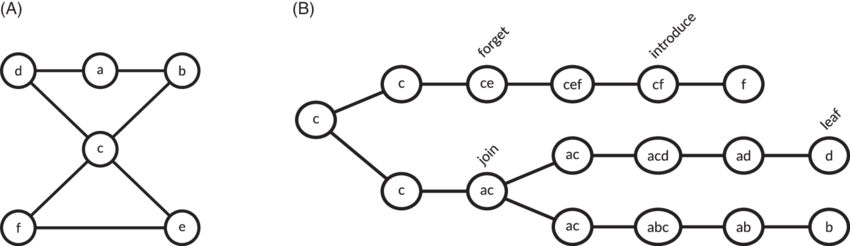
\includegraphics[width=0.80\textwidth]{./assets/nice_tree_decomposition.png}
	\end{center}
	\caption[Nice tree decomposition]{An example of a nice tree decomposition with width three~\cite{nice_tree_decomposition_img}.
		In (A) you can see the decomposed graph, in (B) the nice tree decomposition
		with \LeafNode{}s on the right and the \RootNode{} on the left.
	}%
	% \label{fig:nice_tree_decomposition}
\end{figure}
\todo[inline]{Do in Tikz or SVG, maybe}

Note that a vertex \( v \in V(G) \) can be introduced multiple times,
but forgotten only once.
By \( V_t, t \in T \), we denote the set of vertices introduced by \( t \)
and all its child nodes.

\begin{lemma}[\cite{book_parametrized_algorithms}]
	Any tree decomposition of width at most \( k \) can be converted to
	a nice tree decomposition of width at most \( k \)
	in time \( O(k^2 \cdot \max(|V(T)|, |V(G)|)) \).
	The nice decomposition tree has at most \( O(k|V(G)|) \) nodes.
\end{lemma}

The problem of finding treewidth is NP-complete~\cite{tree_width_np_complete}.
Luckily, the problem is studied a lot and
there exist efficient approximation algorithms~\cite{tree_width_approximation}.
We consider nice tree decompositions as given along with a graph
and do not consider runtime required to find it.

In \IntroduceVertexNode{}, all the edges connecting it
to vertices in \( X_{t^\prime} \) are usually considered while processing \( t \).
%
For some problems it is beneficial to divide this operation further.
First a vertex is added with no edges using a \IntroduceVertexNode{}
and later all the edges corresponding to the vertex are added using new \IntroduceEdgeNode{}s.
We define an edge bag \( Y_t, t \in T \) similarly as vertex bags \( X_t \).
%
Let \( t^\prime \) be a direct ancestor of \( t \).
For \IntroduceVertexNode{}, we define \( Y_t = Y_{t^\prime} \).
For \ForgetVertexNode{} forgetting vertex \( v \),
we define \( Y_t = Y_{t^\prime} \setminus \{ e \in E(G) \mid v \in e\} \).
For a \JoinNode{}, the condition \( Y_t = Y_{t_1} = Y_{t_2} \) must hold.
%
By \( E_t, t \in T \), we denote the set of edges introduced by \( t \)
and all its child nodes.
By \( G_t, t \in T \), we mean the graph \( G_t = (V_t, E_t) \).
%
\begin{definition}[\IntroduceEdgeNode{}~\cite{book_parametrized_algorithms}]
	A node \( t \), labeled with an edge \( e = \{u, v\} \in E(G) \)
	such that \( u, v \in X_t \) and with exactly one child \( t^\prime \)
	such that \( X_t = X_{t^\prime} \), \( Y_t = Y_{t^\prime} \cup \{e\} \).
	We say that \( e \) is \emph{introduced} by \( t \).
\end{definition}
%
Each edge can be introduced at most once.

For edge \( \{u, v\} \) we can transform a nice tree decomposition \( T \)
by adding \IntroduceEdgeNode{}s \( t \) above \IntroduceVertexNode{}s of \( u, v \)
and bellow \ForgetVertexNode{}s of \( u, v \) in \( T \).

%
\begin{lemma}
	For each \JoinNode{} \( t \in T \) with children \( t_1, t_2 \)
	it holds that \( Y_t = \emptyset \).
\end{lemma}
%
\begin{proof}
	Assume there is an edge \( e = \{u, v\} \in Y_t \).
	As each edge can be added and removed exactly once
	and in a \JoinNode{} \( t \) both bags need to be the same,
	edge \( e \) must have been introduced in both \( t_1 \) and \( t_2 \).
\end{proof}
%

%%%%%%%%%%%%%%%%%%%%%%%%%%%%%%%%%%%%%%%%%%%%%%%%%%%%%%%%%%%%%%%%%%%%%%%%%%%%%%%%
\section{Monadic second-order logic}

Monadic second-order logic~(\MSO{}) on graphs is a logical system based on
well known predicate logic.
In the world of parametrized algorithms,
it often comes handy --- if we are able to represent a problem using~\MSO{},
then there exists an FPT algorithm parametrized by treewidth
that can solve the problem~\cite{tree_width_mso}.

\subsection{Introduction to~\MSO{}}

In the following paragraphs we paraphrase and simplify formal definition
from~\cite{book_parametrized_algorithms}.
We presume that reader is already familiar with first-order predicate logic.
Second-order predicate logic as an extension of first-order predicate logic,
that adds option to quantify over predicates.

\MSO{}~is an realization of second-order predicate logic.
\todo[inline]{TODO Convert to footnote, currently, it raises exceptions in NVim}
\emph{
	% \footnote{
	We need second-order logic as quantification over subsets of vertices or edges
	corresponds to quantification over predicates defining the subsets.
	Without this requirement, we could talk
	about the monadic first-order logic \( \text{MSO}_1 \).
}

Formulas can be formed from
variables, constants, predicates,
boolean operations \( \lnot, \land, \lor, \Rightarrow, \Leftrightarrow \)
and quantifiers \( \forall, \exists \).
Complex formulas are created recursively from atomic formulas
by applying schema related to each operation or quantifier.
This process is the same as in the first-order predicate logic.

Formulas of \MSO{} can use four types of variables:
for single vertices, single edges, subsets of vertices, and subsets of edges.
An evaluation function is a mapping from variables to truth assignments.
By \( u^G \) we denote evaluation of variable \( u \) in graph \( G \)
for some model \( \mathcal{G} \) (a tuple of evaluation function and \( G \)).
In \MSO{} to form atomic formulas, we allow only following base predicates:
%
\begin{itemize}
	\item For \( u \) representing a vertex (edge) variable
	      and \( X \) is a vertex (edge) subset,
	      we can write formula \( u \in X \).
	      For \( G \) the formula is true if \( u^G \in X^G \) is true.
	\item Let \( u \) be a vertex variable and \( e \) be an edge variable,
	      then we can write formula \( \inc (u, e) \).
	      For \( G \) the formula is true if \( u^G \) is an endpoint of \( e^G \).
	\item For any two variables \( u, v \) of the same type we can write \( u = v \).
	      For \( G \) the formula is true if \( u^G = v^G \).
\end{itemize}
%
We also allow simplifications like \( \ne, \not\in \).
As obvious from types of variables, we can quantify over vertices, edges,
subsets of vertices and subsets of edges.

It is beneficial to define auxiliary predicates to simplify our work.
We follow by some examples and simplifications taken from~\cite{book_parametrized_algorithms}.
First we show predicate \( \text{adj} \) represents if two vertices are adjacent.
%
\begin{align*}
	\text{adj}(u, v) \coloneqq (u \ne v) \land (\exists e \in E : \inc (u, e) \land \inc (v, e))
\end{align*}
%
For a graph \( G = (V, E) \) we can represent connectivity of its induced subgraph
on vertices \( X \subseteq V \) with the following predicate~\cite{book_parametrized_algorithms}.
%
\begin{align*}
	\text{connected}(X) \coloneqq \, &
	\forall Y \subseteq V : \Big(
	(
	\exists u \in X : u \in Y \land
	\exists v \in X : v \not\in Y
	)
	\\ &
	\Rightarrow
	(
	\exists u, v \in X : \text{adj}(u, v) \land u \in Y \land v \not\in Y
	)\Big).
\end{align*}
%
Notice that we used our previously defined predicate as an alias.
For \( X = V \) the formula would read as:
``For each separation of a graph, there exists an edge connecting both partitions''.

\subsection{Relation to treewidth}

In the following, for a formula \( \phi \) by \( \|\phi\| \)
we denote the length of the encoding of \( \phi \) as a string.
%
\begin{theorem}[Courcelle's theorem,~\cite{tree_width_mso,book_parametrized_algorithms}]%
	\label{theorem:courcelles_theorem}%
	Assume that \( \phi \) is a formula of \MSO{} and
	\( G \) is an \( n \)-vertex graph equipped
	with evaluation of all the free variables of \( \phi \).
	Suppose, moreover, that a tree decomposition of \( G \) of width \( k \) is provided.
	Then there exists an algorithm that verifies whether \( \phi \)
	is satisfied in \( G \) in time \( f (\|\phi\|, k) \cdot n \),
	for some computable function \( f \).
\end{theorem}
%
If we are given an optimal tree decomposition, or we manage to find good enough
approximation, we know that we can decide any formula in \MSO{} in a time
polynomial in \( n \), we are given no guaranties about the complexity of \( f \).

\subsection{Expressing NAC-colorings using \MSO{}}

In this section we present results from our paper previous~\cite{my_paper}.
We start by defining other auxiliary predicates:
%
\begin{itemize}
	\item For \( V \) all vertices and \( E \) subset of edges we define predicate
	      %
	      \begin{align*}
		      \text{deg2}(E) \coloneqq \,
		       & \forall e \in E : \forall v \in V : \inc (v, e) \Rightarrow \Big( \exists e^\prime \in E : \\
		       & \big( \inc (v, e^\prime) \land e \ne e^\prime \land (\forall e^{\prime\prime} \in E :
				      \lnot \inc (v, e^{\prime\prime}) \lor e^{\prime\prime} \not\in \{e, e^\prime\}) \big) \Big).
	      \end{align*}
	      %
	      The predicate says that all vertices incident to edges in \( E \) have degree two.
	      %
	\item For \( V \) subset of vertices and \( E \) subset of edges we define predicate
	      %
	      \begin{align*}
		      \text{incident}(V, E) \coloneqq \,
		       & (\forall v \in V : \exists e \in E : \inc (v, e))                                                 \\
		       & \land (\forall e \in E : \exists v_1, v_2 \in V : v_1 \ne v_2 \land \inc (v_1) \land \inc (v_2)).
	      \end{align*}
	      %
	      The predicate says that \( V \) are vertices of the subgraph induced by \( E \)
	      and that \( E \) are edges of the subgraph induced by \( V \).
	      %
	\item For \( E \) subset of edges we define predicate
	      %
	      \begin{align*}
		      \text{cycle}(E) \coloneqq \,
		      \big( \exists X \subseteq V : \text{incident}(X, E) \land \text{connected}(X) \big)
		      \land \text{deg2}(E).
	      \end{align*}
	      %
	      The predicate says that edges \( E \) form a cycle.
	      %
	\item For \( E_1, E_2 \) subsets of edges we define predicate
	      %
	      \begin{align*}
		      \text{partition}(E_1, E_2) \coloneqq \, & (\exists e_1, e_2 \in E : e_1 \in E_1 \land e_2 \in E_2 )    \\
		                                              & \land (\forall e \in E : e \in E_1 \lor e \in E_2 )          \\
		                                              & \land (\forall e \in E : e \not\in E_1 \lor e \not\in E_2 ).
	      \end{align*}
	      %
	      The formula reads as: ``Both the partitions are not empty,
	      and each edge is in exactly one of the partitions''.
	\item For \( C, E_\red, E_\blue \) subsets of edges we define predicate
	      %
	      \begin{align*}
		      \text{NACcond}(C, E_\red, E_\blue) \coloneqq \,
		       & C \subseteq E_\red \lor C \subseteq E_\red
		      \\
		       & \lor (\exists e_1, e_2, e_3, e_4 \in E :
		      e_1 \ne e_2 \land e_3 \ne e_4
		      \\
		       & \qquad \land e_1, e_2 \in E_\red \land e_3, e_4 \in E_\blue ).
	      \end{align*}
	      %
	      The predicate says that the cycles \( C \) is not an almost cycle.
	      %
\end{itemize}
%

With the predicates ready, we can proceed approach to the theorem.
%
\begin{theorem}[\cite{my_paper}]
	The problem of existence of a NAC-coloring is fixed parameter
	tractable when parametrized by treewidth.
\end{theorem}
%
\begin{proof}
	We can express the NAC-coloring problem
	as a formula \( \phi \) in \MSO{} as follows:
	%
	\begin{align*}
		\exists E_\red, E_\blue \subseteq E : \,
		 & \text{partition}(E_\red, E_\blue)                                                                 \\
		 & \land \big(\forall C \subseteq E : \text{cycle}(C) \land \text{NACcond}(C, E_\red, E_\blue) \big)
		.
	\end{align*}
	%
	By \Cref{theorem:courcelles_theorem},
	there exists an FPT algorithm parametrized by treewidth
	that can resolve \( \phi \) and therefore resolve the question whenever a graph has a NAC-coloring.
\end{proof}
%
The proof shows us that there exists such an algorithm,
but it does not give us explicit steps to follow
(even tough they can be deduced from the original proof of \Cref{theorem:courcelles_theorem}).
Still, the complexity guaranties of the algorithm are not very clear.
In the following section we define our
own FPT algorithm that solves the NAC-coloring problem
while not relying on~\MSO{}.

\section{FPT algorithm}

In this section we first introduce the core idea of the algorithm,
go through each type of node in a tree decomposition and
determine the complexity of the algorithm.
Lastly, we optimize the algorithm by empowering using monochromatic components.

Our algorithm is in its core similar to Steiner tree search algorithm
as described in~\cite{book_parametrized_algorithms} as both the problems require connectivity
among vertex partitions. Unlike in the Steiner tree search algorithm,
our state space is even larger and all the operations work significantly differently.

Before we start, we define some terms that will come useful soon.
%
\begin{definition}[Bridge, Neighboring parts]
	For a graph \( G \) with NAC-coloring \( \delta \)
	and two distinct connected components
	with vertices \( U \) and \( V \)
	in \( G[\Ered] \), resp. \( G[\Eblue] \),
	a \emph{bridge} is an edge \( e = \{u, v\} \in E(G) \)
	such that \( u \in U \land v \in V \).
	%
	The components are \emph{neighboring} if there exists
	a bridge for these two components.
\end{definition}
%

First we want to build the intuition for the upcoming operations.
Let us have a graph \( G \) and all the NAC-colorings of the graph \( \nac{G} \).
Let us add an edge \( e = \{u, v\}, e \not\in E(G) \) to form graph~\( G^\prime \).
We want to obtain \( \nac{G^\prime} \) based on \( \NAC (G) \).
%
Let us have \( \delta \in \nac{G} \),
we want to extend it to \( \delta^\prime \) where w.l.o.g.\ \( \delta^\prime(e) = \blue \).
Coloring \( \delta^\prime \) is a NAC-coloring unless an almost cycle is formed in \( G^\prime \).
In that case one of the following cases must be true:
%
\begin{itemize}
	\item Both vertices \( u, v \) are in the same connected component in \( G[\Ered] \).
	      An almost cycle is formed
	      from \( \red \) \( u \)-\( v \)-path in the connected component
	      and edge \( e \) with \( \blue \) color.
	\item Vertices \( u, v \) lay in different connected components in \( G[\Eblue] \)
	      and there is a \( \red \) colored edge connecting some vertices from the components.
	      We call such an edge \emph{bridge}.
	      An almost cycle is formed from \( \blue \) paths in each component,
	      the \( \red \) bridge and \( \blue \) edge \( e \).
\end{itemize}
%
In all other cases an almost cycle cannot be formed by adding \( \blue \) colored edge \( e \).
Note that a vertex cannot be in multiple connected component for the given color
as this fact would mean that both the components are not maximal.

To create \( \nac{G^\prime} \), we extend the colorings
in \( \nac{G} \cup \{ \delta_\red \} \), where \( \delta_\red \)
colors all the edges in \( G \) with \( \red \) color.
We do likewise for the case when \( e \) is colored \( \red \).
Then we keep only the colorings that did not form an almost cycle.

In the following sections
we work with a nice tree decomposition \( T \) with treewidth \( k \)
of a graph \( G \).
The algorithm works only for graphs with at least one edge.

We define an \emph{almost NAC-coloring}
as a \( \red \)-\( \blue \) edge coloring such that there
are no almost cycles formed. The conditions are the same as for NAC-coloring
except that the surjectivity criterion is dropped.
We use almost NAC-coloring for the rest of the section.
Later when output is read in a \RootNode{},
we switch back from almost NAC-colorings to NAC-colorings.

\todo[inline]{Make sure all the mentions of ``factorization'' are removed.}

\emph{Dynamic programming} is a well-known technique for solving problems
where the problem can be subdivided into smaller sub-problems.
Usually, some base cases are solved trivially and then a sub-problem
is solved based on the solution of its smaller sub-problems.
Often it is a case, that a smaller sub-problem is solved multiple times
as it is a part of multiple larger sub-problems.
Its result is therefore cached and reused reducing the running time.
There are many popular dynamic programming algorithms
like \textsc{Edit Distance}, \textsc{Matrix Chain Multiplication} or \textsc{Longest Common Subsequence}.

We define a state space \( S \) of \emph{states}
that will be used by our cache in our dynamic programming algorithm.
We denote all partitions of a set \( X \) by \( \mathcal{F}(X) \).
Note that it always holds that \( \emptyset \in \mathcal{F}(X) \).

%
\begin{definition}[State space]
	Let \( t \in T \) be a node in the nice tree decomposition tree and
	\Xt{} be a bag of vertices.
	% where with \( l \le k+1 \) vertices
	%
	A state is formed by a tuple \( s = (P_\red, R_\red, P_\blue, R_\blue) \)
	where \( P_\red \in \mathcal{F}(X)\), resp. \( P_\blue \), is a partition of \Xt{}
	and \( R_\red\), resp. \(R_\blue \), is a symmetric irreflexive relation
	on parts in \( P_\red\), resp. \(P_\blue \).
	%
	For \( t \), all such states on \Xt{} form the \emph{state space} \( S_t \).
\end{definition}
%
Partitions \( P_\red, P_\blue \) represent vertices
that are in the same connected component in the subgraph of \( G_t \)
induced by edges of the specified color.
It is sort of a projection of NAC-colorings of \( G_t \) narrowed to \( X_t \)
Relations \( R_\red, R_\blue \) represent
whenever the connected components are neighboring.
This plays major role for detecting almost cycles.
%
An almost NAC-coloring \( \delta \) is \emph{consistent} with a state \( (P_\red, R_\red, P_\blue, R_\blue) \in S_t \)
if \( \red \) and \( \blue \) connected components of \( \delta \) form \( P_\red \) and \( P_\blue \)
when intersected with \( X_t \) and
there are bridges between the components as in \( R_\red \) and \( R_\blue \).
%
Note that the state space is somewhat large, we evaluate the size in~\Cref{sec:fpt_time_complexity}.

For the following definitions, lemmas, proofs and theorems, let us fix
a nice tree decomposition \( T \).

\begin{definition}[Cache function]
	Let us have a mapping \( c: \mathcal{S} \to \N \)
	where \( \mathcal{S} = \{ (t,s): t \in T, s \in S_t \} \).
	If it holds, that for \( c(t, s) \) maps to the number of almost NAC-colorings of \( G_t \)
	consistent with \( s \), we call \( c \) a \emph{cache function}.
	By \emph{cache entry} we denote a pair \( (t, s) \in \mathcal{S} \).
\end{definition}
%
\begin{observation}
	For each almost NAC-coloring \( \delta \) on \( G_t \)
	there is single state \( s \in S_t \) consistent with it.
	It holds that \( |\nac{G_t}| + 2 = \sum_{s \in S_t} c(t, s) \).
\end{observation}

In the following sections we show how to construct a cache function \( c \)
based on values of child nodes.
We make sure that invalid states that cannot occur by applying our operation (non-valid states)
get zero cache entry value as they cannot represent any almost NAC-coloring.
We prove the algorithm's correctness by induction.
The base case is for \LeafNode{}s, for other nodes we split the reasoning for cases where
there is or is not at least one edge in \( G_t \).
Next few lemmas work as follows: for a state \( s \in S_t \)
we derive states \( s^\prime \in S_{t^\prime} \) from whose cache entry \( (t, s) \)
can be computed based on values \( c[t^\prime, s^\prime] \).

\begin{lemma}
	Let us have a \LeafNode{} \( t \in T \).
	It holds that \( c[t, s] \coloneqq 0 \) for all \( s \in S_t \).
\end{lemma}
%
\begin{proof}
	There are no edges as \( X_t \) has no edges.
	By definition of the cache function \( c \) must hold \( 0 \)
	for each state.
\end{proof}
%
Note that for \( t \in T \) \LeafNode{},
the only state in \( S_t \) is \( (\emptyset, \emptyset, \emptyset, \emptyset) \).

\begin{lemma}
	Let an \IntroduceVertexNode{} \( t \in T \) be
	the only parent of \( t^\prime\) in \( T \) and let \( s \in S_t \).
	Let \( v \) be the only vertex in \( X_t \setminus X_{t^\prime} \).
	%
	If there is no edge in the graph \( G_t \), then \( c[t, s] \coloneqq 0 \).
	%
	Otherwise, we define cache function value for \( s=(P_\red, R_\red, P_\blue, R_\blue), s \in S_t \)
	for \( a \in \{\red, \blue\} \) as:
	%
	\begin{align*}
		c[t, s] & \coloneqq
		\begin{cases}
			0,                                                                                       & \text{if } \exists a : \{v\} \not\in P_a,                    \\
			0,                                                                                       & \text{if } \exists a \exists p \in P_a : (\{v\}, p) \in R_a, \\
			c[t^\prime, (P_\red \setminus \{\{v\}\}, R_\red, P_\blue \setminus \{\{v\}\}, R_\blue)], & \text{otherwise},
		\end{cases} \\
	\end{align*}
\end{lemma}
%
The state \( (P_\red \setminus \{\{v\}\}, R_\red, P_\blue \setminus \{\{v\}\}, R_\blue) \)
represents the state where \( v \) is not present in any connected component
and where the same connected components are neighbors.
%
\begin{proof}
	By definition, there are no almost NAC-colorings
	in \( G_t \) if \( G_t \) has no edges.
	%
	If vertex \( v \) is in a part of \( P_\red \) or \( P_\blue \) with other vertices,
	the cache value must be zero as \( v \) is an isolated vertex in \( G_t \)
	and therefore no almost NAC-colorings consistent with such state exists.
	Therefore, there must be a part \( \{v\} \).
	%
	Also, as \( v \) is an isolated vertex in \( G_t \), there cannot be a bridge
	connecting this and another component.
	Thus, for all states where there exists
	a part neighboring \( \{v\} \), there are no consistent almost NAC-colorings
	and therefore the cache value must be also zero.
	Remember that \( R_\red, R_\blue \) are relations --- sets of pairs.
	%
	By adding a vertex to \( G_{t^\prime} \), we cannot create new almost cycles
	or extend existing almost NAC-colorings as no new edge was added.
	Therefore, the number of almost NAC-coloring for a state \( s \) must be the same
	as for the state \( (P_\red \setminus \{\{v\}\}, R_\red, P_\blue \setminus \{\{v\}\}, R_\blue) \).
\end{proof}
%
To summarize, already computed values are propagated to the consistent states.

\begin{lemma}
	Let a \ForgetVertexNode{} \( t \in T \) be
	the only parent of \( t^\prime \in T \) and let \( s \in S_t \).
	Let \( v \) be the only vertex in \( X_{t^\prime} \setminus X_t \).
	%
	If there are no edges in the graph \( G_t \), then \( c[t, s] \coloneqq 0 \).
	%
	Otherwise, we define the cache function value for \( s=(P_\red, R_\red, P_\blue, R_\blue) \)
	for \( a \in \{\red, \blue\} \) as:
	%
	\begin{align*}
		c[t, s]                        & \coloneqq \sum_{s^\prime \in S^\prime} c[t^\prime, s^\prime],                                                                                                         \\
		\text{where}                                                                                                                                                                                           \\
		m(p)                           & \coloneqq p \setminus \{v\},                                                                                                                                          \\
		M(P)                           & \coloneqq \{m(p) \mid p \in P \} \setminus \{\emptyset\},                                                                                                             \\
		\mathcal{P^\prime}_a           & \coloneqq \{ P_a^\prime \in \mathcal{F}(X_{t^\prime}) \mid M(P_a^\prime) = P_a \},                                                                                    \\
		\mathcal{R^\prime}(P_a^\prime) & \coloneqq \{ R_a^\prime \subseteq P_a^\prime \times P_a^\prime \mid \forall (p_1, p_2) \in R_a^\prime :                                                                                                    \\
		                               & \qquad (m(p_1), m(p_2)) \in R_a \lor m(p_1) = \emptyset \lor m(p_2) = \emptyset \},                                               \\
		S^\prime                       & \coloneqq \{(P_\red^\prime, R_\red^\prime, P_\blue^\prime, R_\blue^\prime) \mid P_a^\prime \in \mathcal{P^\prime}_a, R^\prime \in \mathcal{R^\prime}(P_a^\prime)  \}. \\
	\end{align*}
	\( m(p) \) denotes deleting the vertex \( v \) from part \( p \).
	\( M(P) \) denotes deleting the vertex \( v \) from all the parts in partition \( P \)
	--- if \( \{v\} in P \), resulting \( \emptyset \) is also cleared.
	\( \mathcal{P^\prime}_a \) denotes all the partitions such that removing \( v \) from them gives \( P_a \).
	\( \mathcal{R^\prime}(P_a^\prime) \) denotes all the relations \( R_a^\prime \)
	for \( P_a^\prime \in \mathcal{P^\prime}_a \) that correspond with \( R_a \) when \( v \) is removed
	--- parts are updated or relations to \( \{v\} \) is removed.
	\( S^\prime \) are all the states that correspond to state \( s \).
\end{lemma}
%
%
\begin{proof}
	If there were no edges in \( G_t \), none were added by a \ForgetVertexNode{}.
	Therefore, \( c[t, s] \coloneqq 0 \).
	%
	If state is invalid, all the previous states that collapse into it by removing \( v \)
	are also invalid, therefore the resulting value is zero.
	%
	If \( v \) did not share a connected component with other vertices,
	and if we later add an edge \( e = \{u, v\}, u, v \in X_t \) to the graph,
	no almost cycle using \( v \) cannot be created as entering and leaving the component
	requires more than one edge of each color.
	%
	Lastly if \( v \) shares a connected component with other vertices,
	and an almost cycle passing through \( v \) is created in the future,
	in can be rerouted to pass through other vertices of the connected component,
	If not there is a bridge incident to \( v \), such information if passed
	further using neighboring relation and such cycle will be found.
	Therefore, the number of NAC-colorings stays the same if we remove \( v \)
	from  partitions.
	%
	The resulting cache entry holds values from both the state types.
\end{proof}
%

\subsection{\IntroduceEdgeNode}

Suppose that \( t \in T \) is
the only parent of \( t^\prime \in T \).
It holds that \( X_t = X_{t^\prime} \),
let \( e = \{u, v\} \) be the only edge added in the step, \( e \in T_t \setminus Y_{t^\prime} \).
We will discuss all the possible cases that must be fulfilled for both colors,
otherwise the resulting value for the state given is zero.
Interactions between components of different colors are of no interest for us.
We state conditions for a single color, w.l.o.g.\ let the edge \( e \) be \( \blue \):
%
\begin{description}
	\item[Edge lies in a \( \blue \) connected component]
	      In this case there is no risk of an almost cycle being created.
	\item[Edge lies in a \( \red \) connected component]
	      In this case an almost cycle is trivially created,
	      therefore this is not allowed.
	\item[Edge connects two neighboring \( \blue \) connected components]
	      This again causes an almost cycle to be created.
	\item[Edge connects two neighboring \( \red \) connected components]
	      This causes no harm as cycle with two \( \blue \) edges is created.
	\item[Edge connects two non-neighboring \( \blue \) connected components]
	      This operation is not allowed as both the components
	      are now connected using this edge.
	\item[Edge connects two non-neighboring \( \red \) connected components]
	      This is not allowed as bot the components
	      are neighbors with \( e \) being the new bridge.
\end{description}
%
Note that both the conditions need to pass.
One holds for the \( \red \) subgraph, the other for \( \blue \).

Now we state how the cached values are computed for cases when
the previous conditions pass for both the colors.
Resulting cache entry is sum of multiple states from the child node
\( t^\prime \) that collapse into the new valid state
as some components are joined,
and some neighboring relations are created:
%
\begin{description}
	\item[Edge lies in a \( \blue \) connected component]
	      First we query the previous cache state with
	      the same partition and neighbors state.
	      Then we also need to add states where
	      both the components were not neighbors as no almost cycle was created
	      and both the separate connected components
	      are now joined into a single component.
	      We denote \( \blue \) components of such state
	      as \( P_\blue^\prime \) and \( R_\blue^\prime \).
	      Note, that other relations between partitions need to match.
	\item[Edge connects two neighboring \( \red \) connected components]
	      Result is a sum of previous states with the same partitioning as \( P_\red \),
	      for first query we use \( R_\red \),
	      and then we add query of \( R^\prime_\red = R_\red \setminus \{(c(u), c(v)), (c(v), c(u))\} \)
	      (with the neighbor constraint removed).
\end{description}
%

The resulting cache for \( \blue \) color is then computed as follows:
%
\begin{align*}
	c_\blue[t, s] & = c[t^\prime, (P_\red, R_\red, P_\blue, R_\blue)]                      \\
	              & + c[t^\prime, (P_\red, R_\red^\prime, P_\blue, R_\blue)]               \\
	              & + c[t^\prime, (P_\red, R_\red, P_\blue^\prime, R_\blue^\prime)]        \\
	              & + c[t^\prime, (P_\red, R_\red^\prime, P_\blue^\prime, R_\blue^\prime)]
\end{align*}
%
If some rule was not matched for \( s \) and \( e \) colored \( \blue \)
the cache entry results into \( c_\blue[t, s] = 0 \).

The final entry is \( c[t, s] = c_\red[t, s] + c_\blue[t, s] \).

\subsection{\JoinNode}

Suppose that \( t \in T \) is
the only parent of \( t_1, t_2 \in T \).
It holds that \( X_t = X_{t_1} = X_{t_2} \)
and \( S = S_1 = S_2 \) where \( S_\cdot \) are corresponding cache state spaces.

We create mappings \( M: S_1 \times S_2 \to S \) and \( N: S_1 \times S_2 \to \{0, 1\} \).
Mapping \( M \) maps to the state when connected components of both the states
are joined together and \( N \) states if the given join is valid.

Let \( {(.)}^* \) denote the transitive closure of a set.
For states let us have
% \( s = (P_\red, R_\red, P_\blue, R_\blue), s \in S \),
\( s_1 = (P_{1,\red}, R_{1,\red}, P_{1,\blue}, R_{1,\blue}), s_1 \in S_1 \) and
\( s_2 = (P_{2,\red}, R_{2,\red}, P_{2,\blue}, R_{2,\blue}), s_2 \in S_2 \).
Let \( a \in \{\red, \blue\} \),
We take original relations \( O_{1, a}, O_{2, a} \)
from which \( P_{1, a}, P_{2, a} \) were factorizes.
We set
%
\begin{align*}
	O_a & \coloneqq {(O_{1, a} \cup O_{2, a})}^* \\
	P_a & \coloneqq \mathcal{F}_{O_a}(X_t)
\end{align*}
%
where \( \mathcal{F}_O(X) \) stands for factorization of \( X \)
according to relation \( O \). This operation represents merging connected
components from both the states. No NAC-coloring related checking is performed yet.

We continue with neighbors relation. We drop connections that related components
that were merged (we will get back to them soon).
Let for \( i \in {1, 2} \)
%
\begin{align*}
	R_{i,a}^\prime & \coloneqq \{(p_1, p_2) \mid p_1, p_2 \in P_a,                                                                                                            \\
	               & \qquad \exists p_1^\prime, p_2^\prime \in P_{i,a} : (p_1^\prime, p_2^\prime) \in R_{i,a} \land p_1^\prime \subseteq p_1 \land p_2^\prime \subseteq p_2\}
\end{align*}
%
and w.l.o.g.\ let \( R_a \coloneqq R_{1,a} \).
Then we define mapping \( M \) as \[ M(s_1, s_2) = (P_\red, R_\red, P_\blue, R_\blue). \]

We follow with mapping \( N \) that states if the merge done by \( M \) is valid.
First, sates that provide different guaranties
(\( R_{1,a}^\prime \not= R_{2,a}^\prime \)) about neighboring components
among the components in the final state are unsuitable.
Now we need to validate that we did not create an almost cycle by checking
neighboring relations in \( R_{1,a} \) among components from \( P_{1,a} \)
that will be merged because of \( P_{2,\red}, P_{2,\blue} \).
The same follows the other way.

The rest of the statement follows similar in introduce edge node proof.
The check is done once again for both the colors.
Let us go through cases how can an almost cycle be created.
Suppose the only edge with different color is colored \( \red \).
Then there must exist a \( \blue \) path. If the path spans only using vertices
in \( V_{t_1} \), the cache entry must hold zero as no NAC-coloring can come
from \( s_1 \). This case is of not interest to us.
Therefore, the \( \red \) edge must be
a bridge connecting two \( \blue \) components in \( P_{1,\blue} \) and
the path has to also span trough vertices in \( V_{t_2} \).
Such vertices have to share the same connected \( \blue \) component in \( P_{2,\blue} \).
This happens if and only if there is a neighboring pair of components in \( P_{1,\blue} \)
that can be connected by a \( \blue \) path in \( P_{2,\blue} \).

To formalize let \( a \in \{\red, \blue \}  \) and \( b \in \{\red, \blue \} \setminus \{a\} \).
Let \( \mathcal{P} \subseteq P_{1, a} \)
and \( p \in P_{a} \) such that \( \bigcup_{p^\prime \in \mathcal{P}} p^\prime = p \).
If there exists \( p_1, p_2 \in \mathcal{P} : (p_1, p_2) \in R_{1, a} \),
this state is not acceptable as an almost cycle is created
using a \( \red \) bridge connecting \( p_1 \) and \( p_2 \).

This is the only way an almost cycle can be created as no edges are added.
Note that each vertex in \( X_t \) is part of both \( \red \) and \( \blue \)
components even if the components have just a single vertex.
All the checks for both sides (\( 1, 2 \)) and colors are run and
if a single one of them fails, the states pair is considered bad.
We denote set of such bad states as \( \mathcal{B}, (s_1, s_2) \in \mathcal{B} \).

%
\begin{align*}
	N(s_1, s_2) =
	\begin{cases}
		0, & \text{if } (s_1, s_2) \in \mathcal{B}                  \\
		0, & \text{if } \exists a : R_{1,a}^\prime = R_{2,a}^\prime \\
		1, & \text{otherwise}
	\end{cases}
\end{align*}
%

Lastly we show formula to compute cache entries based on previously stated mappings.
It comes from the same idea as coloring product where all the resulting colorings
are NAC-colorings. The size of such product is multiple of sizes of the original subgraphs.
%
\begin{align*}
	\mathcal{S}(s) & \coloneqq \{(s_1, s_2) \mid M(s_1, s_2) = s \}                                                     \\
	c[t, s]        & \coloneqq \sum_{(s_1, s_2) \in \mathcal{S}(s)} N(s_1, s_2) \cdot c[t_1, s_1] \cdot c[t_{2}, s_{2}]
\end{align*}
%

This finishes our basic dynamic programming algorithm
for counting NAC-colorings of the graph.
The number of NAC-colorings is the only value stored in cache
after the last vertex is forgotten.

\subsection{\LeafNode{}}

Usually \LeafNode{} is the simplest one. Here we use a special value,
that needs not trivial explanation.
In leaf nodes \( t \in T \) we work with not nodes as the bag \Xt{} is empty.
The only factorization on an empty set is an empty set.
We assign 1 to the cache entry. This is necessary to start the algorithm.
%
\begin{align*}
	c[t, (\emptyset, \emptyset, \emptyset, \emptyset)] & \coloneqq 1 \\
\end{align*}
%
\begin{proof}
	We proof that 1 is a good decision.
	The parent of a \LeafNode{} \( t_1 \) must be an \IntroduceVertexNode{} \( t_2 \).
	\( t_2 \) now resolves also to only a single almost NAC-coloring.
	As we stated in our graph preconditions, the graph has at least one edge
	and therefore at least two vertices.

	After \( t_2 \) two kinds of nodes can follow.
	Let \( t_2^\prime \) be the unique parent of \( t_2 \).
	If \( t_2^\prime \) is an \IntroduceVertexNode{}, cache entry for state,
	where vertices are disconnected both in \( \red \) and \( \blue \) subgraphs
	gets value 1. Such \IntroduceVertexNode{} can occur multiple times
	while traversing \( T \).
	Let \( t_2^{\prime\prime} \) be the last such node
	(possibly \( t_2 = t_2^{\prime\prime}\) or \( t_2^\prime = t_2^{\prime\prime}\) ).
	Let \( t_3 \) be the parent of \( t_2 \).
	The only options are that \( t_3 \) either is \IntroduceEdgeNode{} or \JoinNode{}.
	If \( t_3 \) is an \IntroduceEdgeNode{} introducing edge \( e = \{u, v\} \),
	the resulting cache entry will store 1 for the state,
	when \( u ,v \) are in the same \( \red  \) component and other vertices are disconnected, or
	when \( u ,v \) are in the same \( \blue \) component and other vertices are disconnected.
	This correctly represents almost NAC-colorings in \( G_{t_3} \).
	If \( t_3 \) is a \JoinNode{}, the number of almost NAC-coloring should not change.
	As the value are multiplied by 1, this precondition holds.
\end{proof}

\subsection{\RootNode{}}

Finally, for \( r \in T \) \RootNode{} and its unique child \( t^\prime \)
we read value from cache entry as follows:
%
\begin{align*}
	\text{output} \coloneqq c[t^\prime, (\emptyset,\emptyset,\emptyset,\emptyset)] - 2.
\end{align*}
%
We need to subtract two as the output of the algorithm are NAC-coloring,
not almost NAC-colorings. Correctness goes from the previous nodes.
From that it can be clearly observed that the algorithm
will never give you up~\cite{never_gonna_give_you_up}.

\subsection{Time complexity}%
\label{sec:fpt_time_complexity}

Bell numbers are defined as the number of factorizations of the set.
They can be upper bounded by \( n^n \), which is what we will use from now on.
\todo[inline]{Reference?}
Recall that \( \forall t \in T : |X_t| \le k+1 \).

First, size of the state space used is upper bounded.
For each color there is up to \( {(k+1)}^{(k+1)} \) factorizations of a bag and
up to \( 2^{\binom(k, 2)} \) neighbors relations.
Total state space size for each bag is therefore bounded by
\( {\big({(k+1)}^{(k+1)} \cdot 2^{\binom{k}{2}} \big)}^2 = {(k+1)}^{2(k+1)} \cdot 2^{2 \binom{k}{2}} \).

We go through all the nodes and state complexity of the operations performed in the node:
\begin{description}
	\item[\IntroduceVertexNode{}]
	      We need to fill a state space and copy previous values into the cache
	      which can be done in constant time per operation,
	      so the time complexity corresponds to the state space size:
	      \( {k}^{O(k)} \cdot 2^{O(k)} \cdot O(1) \).
	\item[\ForgetVertexNode{}]
	      Even if the operation seams complex, we just need to traverse the state space
	      and create target state after \( v \) is removed. This can be done in \( O(k) \) time
	      per state, total complexity therefore is
	      \( {k}^{O(k)} \cdot 2^{O(k)} \cdot O(k) \).
	\item[\IntroduceEdgeNode{}]
	      The state space is iterated again, and we run few simple checks and cache key constructions
	      that can be run in \( O(k) \) time, therefore the final complexity stays the same
	      \( {k}^{O(k)} \cdot 2^{O(k)} \cdot O(k) \).
	\item[\JoinNode{}]
	      We iterate through product of state spaces,
	      so the size of the new spate space is power of two
	      of the otherwise used state space size.
	      This hides into the big \( O \) notation.
	      Checks run checking for almost cycles can be run in time \( O(k^2) \).
	      Thus, the final		complexity is
	      \( {k}^{O(k)} \cdot 2^{O(k)} \cdot O(k^2) \).
\end{description}

There are \( O((n+m)k) \) nodes in \( T \).
The final complexity of the algorithm is therefore
\( {k}^{O(k)} \cdot O(n^2) \).
\todo[inline]{Check number of nodes in \( T \)}

\subsection{\IntroduceVertexWithEdgesNode{}}

As also described above, FPT algorithms parametrized by treewidth
often use \IntroduceVertexNode{} that also introduces edges,
for this section we call this node \IntroduceVertexWithEdgesNode{}.
The original algorithm can be modified to use this node.
We outline the proof of correctness of such operation and the show
that it is actually asymptotically slower than the originally proposed algorithm.

The previous expression tree is modified by
replacing every \IntroduceVertexNode{} by \IntroduceVertexWithEdgesNode{}
and removing every \IntroduceEdgeNode{}.
The other nodes including \ForgetVertexNode{} and \JoinNode{} stay unchanged
with no behavior changes.

Let us describe how \IntroduceVertexWithEdgesNode{} processes cache entries.
Before, when a single edge was added,
we checked if there is some constraint violation
--- if an almost cycle was formed.
The same is also done for \IntroduceVertexWithEdgesNode{},
but you can think of the process as
multiple such constrains checked at the same time.

As it is nontrivial and confusing to describe this operation
by using predicate logic, we stick to natural language for simplicity.
Suppose that \( t \in T \) is
the only parent of \( t^\prime\) in \( \mathcal {T} \).
Let \( v \) be the only vertex in \( X_t \setminus X_{t^\prime} \).
Let \( E_\Delta \) be edges added,
\( E_\Delta = \{ \{ u, v \} \mid u \in X_t \} \cap E(G) \).
Let us have set \( \Lambda \) of all \( \red \)-\( \blue \)-colorings on \( E_\Delta \).
We define mapping \( m: S^\prime \times \Lambda \to S \)
that represents how state changes for a coloring of edges in \( E_\delta \).
Let us have some \( s^\prime \in S^\prime \) and \( \lambda \in \Lambda \)
and \( m(s^\prime, \lambda) = s, s \in S \).

Vertices \( u, v \in X_t \) share the same \( \blue \) connected component if either:
%
\begin{itemize}
	\item They shared the same connected component in \( s^\prime \).
	\item There is a \( \blue \) path in \( E_\Delta \) with coloring \( \lambda \).
\end{itemize}
%
Note that \( \blue \) connected components created by following this procedure
are same as in \( s^\prime \) or merged \( \blue \) components of \( s^\prime \)
except for \( v \) as it is not yet in \( X_{t^\prime} \).
Such \( \blue \) connected components are neighboring if either:
%
\begin{itemize}
	\item They or their predecessors in \( s^\prime \)
	      were neighbors in \( s^\prime \).
	\item There is a path in \( E_\Delta \) with
	      one \( \blue \) and one \( \red \) edge
	      according to coloring \( \lambda \).
	      The \( \red \) edge becomes a bridge.
\end{itemize}
%
Now the same is done for \( \red \).
We ensure that all the rules described in \IntroduceEdgeNode{}
still hold for \( s \). If so, \( c[t, s] \pluseq c[t^\prime, s^\prime] \).
This all is done for each combination in \( S^\prime \time \Lambda \).

For the original algorithm for each \( v \)
\IntroduceEdgeNode{} is used \( |E_\Delta| \) times
and \( \IntroduceVertexNode{} \) once, therefore added complexity for \( v \)
is \( {k}^{O(k)} \cdot 2^{O(k)} \cdot (|E_\Delta| + 1) \).
%
For \IntroduceVertexWithEdgesNode{} we iterate
through all the colorings in \( \Lambda \) for each state.
As size of \( \Lambda \) is \( |\Lambda| = 2^|E_\Delta| \),
the required runtime added for \( v \) is
\( {k}^{O(k)} \cdot 2^{O(k)} \cdot 2^{|E_\Delta|}\)
which is asymptotically higher and therefore slower.

\subsection{Monochromatic components}

Monochromatic components can be used to significantly reduce state space
that needs to be searched. First we introduce state space reduction when
there is an edge in a bag, then we extend the result to multiple edges
sharing the same monochromatic component, and lastly we improve the number of
operations needed in the \IntroduceVertexNode{}.
%
\begin{theorem}
	For \( t \in T \) and an edge \( e = \{u, v\} \) in \( Y_t \).
	Then for states \( s = (P_\red, R_\red, P_\blue, R_\blue), s \in S \) such that
	\( \forall a \in {\red, \blue} \forall p \in P_a : u \in p \Rightarrow v \not\in p \)
	it holds that \( c[t, s] = 0 \).
\end{theorem}
%
%
\begin{proof}
	For contradiction suppose that such state is valid. The edge \( e \)
	has to be either \( \red \) or \( \blue \). Let w.l.o.g.\ \( e \) be colored \( \blue \).
	That means that both \( u, v \) are in the same \( \blue \) connected component.
	But the state \( s \) states that \( u, v \) do not share a \( \blue \) connected component.
	This is contradiction and such state \( s \) is therefore not acceptable
	and the cache entry should store zero.
\end{proof}
%

We extend the result for monochromatic components as follows.
See that this is just a generalization of the previous theorem
as an edge forms a trivial monochromatic class.
%
\begin{theorem}
	For \( t \in T \),
	edges \( E_M \subseteq Y_t \) such that
	they share the same connected monochromatic component
	and vertices \( U \) such that they are end points of the edges in \( E_M \).
	Then for states \( s = (P_\red, R_\red, P_\blue, R_\blue), s \in S \) such that
	\( \forall a \in {\red, \blue} \forall p \in P_a : U \not\subseteq p \)
	it holds that \( c[t, s] = 0 \).
\end{theorem}
%
%
\begin{proof}
	For contradiction suppose that such state is valid. The edges \( E_M \)
	has to be either \( \red \) or \( \blue \).
	Let w.l.o.g.\ edges in \( E_M \) be colored \( \blue \).
	That means that all vertices in \( U \) are in the same \( \blue \) connected component
	and the edges are from a connected monochromatic component.
	But the state \( s \) states that there is a vertex \( u \in U \)
	that does not share a \( \blue \) connected component with the other.
	This is contradiction and such state \( s \) is therefore not acceptable
	and the cache entry should store zero.
\end{proof}
%

Lastly, we describe how \IntroduceVertexWithEdgesNode{} can be optimized.
First, while traversing all the colorings of the edges incident to the added vertex \( E_N \)
we do not try all the color combinations as usual. If there are some edges
in \( E_{t^\prime} \cup E_N \) that are part of a monochromatic component,
the same as above applies. We cannot create a contradicting state with non-zero
cache entry. But by using monochromatic classes
we can enforce that both the edges should always have the same color.
We can also enforce the color by using an edge of the same monochromatic class
that is a part of \( E_{t^\prime} \).
For example if the edge in \( E_{t^\prime} \) is part of a \( \blue \) connected class,
the other edges from the same monochromatic component can be added with
this idea in consideration.


\todo[inline]{Fix monochromatic components notation based on the rest of the thesis}

\subsection{Connectivity}

Along with the cache we can also hold an information about connectivity of
vertices in bags.
%
\begin{definition}[Connectivity map]
	Let \( t \in T \) be a node in a nice tree decomposition tree and
	\Xt{} be a bag of vertices.
	A \emph{connectivity map} \( C_t \) is a factorization of \Xt{}.
	For \( u, v \in V_t \) it holds that
	\( \exists c \in C_t : u \in c \land v \in c \) iff
	\( u, v \) are in the same connected component in \( G_t \).
	A state \( s \in S_t \) is \emph{in conflict} with \( C_t \)
	if \( P_\red \) or \( P_\blue \) are not same or finer that \( C_t \).
\end{definition}
%
We show how connectivity map changes for different types of nodes.
Consider a node \( t \in T \) and its child \( t^\prime \)
or children \( t_1, t_2 \) in case of a \JoinNode{}.
%
For an \IntroduceVertexNode{}
a new connectivity map is obtained as follows:
\( C_t \coloneqq C_t^\prime \cup \{\{ v \}\} \).
%
For a \ForgetVertexNode{}
a new connectivity map is obtained as
\( C_t \coloneqq M(C_t^\prime) \)
where \( M \) is mapping from the \ForgetVertexNode{}
deleting occurrences of forgotten vertex from the factorization given.
%
For an \IntroduceEdgeNode{}
where edge \( \{u, v\} \) is introduced
components of \( u, v \) are merged if they are not merged already.
%
For a \JoinNode{}
connectivity maps \( C_{t_1}, C_{t_2} \) are merged into
a single connectivity map \( C_t \)
the same way as when a \JoinNode{} is processed.
%
For a \LeafNode{}
no vertices are connected yet, so the connectivity map \( C_t = \emptyset \).

With such connectivity map we can not reduce the state space by only considering
factorizations that are finer then the connectivity map.

\subsection{NAC-coloring certificate}

To obtain a NAC-coloring certificate or all the NAC-colorings of the graph
given we need to traverse the cache backwards recursively.
The only step where edges were added to the graph are either \IntroduceEdgeNode{}
or \IntroduceVertexWithEdgesNode{}. In both cases the given cache entry correspond
to some color given to the edge. From the recursive step we can obtain
all the NAC-colorings of \( V_{t^\prime} \) and add our edge.
Note that the whole cache has to be stored in memory the whole time unless
NAC-colorings are materialized while the algorithm runs.
This kills our performance as we process up to \( 2^{O(n^2)} \) colorings
in each node of the tree.

\subsection{Other optimizations}

First it is trivial to see that if the input graph has an articulation,
we can once again run our algorithm on each block of the graph separately
and then multiply the results together to get the final result
while also considering monochromatic colorings of each block.
Note that the same can be done for disconnected graphs.

There is possibility that the algorithm can be further improved by creating
a Monte Carlo algorithm or a linear algebra based algorithm that can run
in \( O(c^k), c \in \N \) time as~\cite{book_parametrized_algorithms} suggests
for problems with connectivity requirements.
This is unfortunately far beyond the scope of this thesis.

\todo[inline]{Cite/Introduce Monte Carlo algorithms}

